\chapter{Implementation}
\section{Development Process}

 \subsection{Initial Architecture Design}
The development process began with a modular architecture designed around four primary components, each with distinct responsibilities and well-defined interfaces:

\begin{itemize}
    \item Camera control system - Handles all camera interactions and image capture
    \item Dataset management - Manages data persistence and organization
    \item Analysis engine - Processes images and performs lens measurements
    \item User interface - Provides user interaction and result visualization
\end{itemize}

\subsection{Camera Integration Development}
The camera integration was implemented in three distinct phases:

\textbf{Phase 1: Basic Camera Communication}
\begin{itemize}
    \item Integration with gphoto2 library for camera control
    \item Implementation of basic camera connection/disconnection logic
    \item Development of camera status monitoring system
    \item Basic error handling and recovery mechanisms
\end{itemize}

\textbf{Phase 2: Advanced Camera Control}
\begin{itemize}
    \item Comprehensive camera settings management
    \item Manual and auto-focus control systems
    \item RAW format capture capabilities
    \item Real-time camera status monitoring
\end{itemize}

\textbf{Phase 3: Robustness Improvements}
\begin{itemize}
    \item Thread-safe camera operations
    \item Automatic camera reconnection handling
    \item Optimized memory management for image capture
    \item Timeout handling for camera operations
\end{itemize}

\subsection{Analysis Engine Development}
The analysis engine evolved through three main stages:

\textbf{Stage 1: Core Analysis Functions}
\begin{itemize}
    \item Raw image processing pipeline implementation
    \item MTF calculation algorithms
    \item Edge detection and analysis systems
    \item Basic lens distortion measurement %todo: prepisat
\end{itemize}

\textbf{Stage 2: Advanced Analysis Features}
\begin{itemize}
    \item Bokeh quality analysis implementation
    \item Chromatic aberration detection algorithms
    \item Vignetting measurement system
    \item Analysis result visualization generation
\end{itemize}

\textbf{Stage 3: Optimization}
\begin{itemize}
    \item Large image processing optimization
    \item Memory usage improvements
    \item Analysis accuracy refinements
    \item Multi-threaded analysis support
\end{itemize}

\subsection{User Interface Evolution}
The user interface development followed an iterative approach:

\textbf{Initial Design}
\begin{itemize}
    \item Basic camera control interface
    \item Simple dataset management
    \item Fundamental result visualization
    \item Basic user feedback mechanisms
\end{itemize}

\textbf{Enhanced Features}
\begin{itemize}
    \item Interactive analysis controls
    \item Advanced dataset organization
    \item Real-time status updates
    \item Analysis progress indicators
\end{itemize}

\textbf{Final Refinements}
\begin{itemize}
    \item UI responsiveness optimization
    \item Comprehensive error reporting
    \item Advanced visualization tools
    \item Batch processing capabilities
\end{itemize}

\subsection{Data Management Implementation}
The data management system was developed in two phases:

\textbf{Core Functionality}
\begin{itemize}
    \item Dataset creation and storage system
    \item Hierarchical file organization
    \item Comprehensive metadata management
    \item Analysis result storage
\end{itemize}

\textbf{Advanced Features}
\begin{itemize}
    \item Dataset import/export functionality
    \item Structured scenario management
    \item Analysis results comparison tools
    \item Data integrity verification systems
\end{itemize}

\subsection{Integration and Testing}
The integration process focused on two main areas:

\textbf{Component Integration}
\begin{itemize}
    \item Systematic core component integration
    \item Interface compatibility validation
    \item Performance optimization
    \item Resource management verification
\end{itemize}

\textbf{Testing Procedures}
\begin{itemize}
    \item Comprehensive unit testing
    \item Component integration testing
    \item Performance load testing
    \item UI functionality verification
\end{itemize}

\subsection{Deployment Considerations}
The final phase addressed deployment requirements:

\textbf{System Requirements}
\begin{itemize}
    \item Hardware compatibility testing
    \item Dependency management
    \item Installation process development
    \item System configuration management
\end{itemize}

\textbf{Documentation}
\begin{itemize}
    \item Technical documentation
    \item User guide creation
    \item API documentation
    \item Installation guides
\end{itemize}

\subsection{Development Tools}
The project utilized modern development tools:

\textbf{Core Technologies}
\begin{itemize}
    \item Python as primary development language
    \item gphoto2 for camera interfacing
    \item OpenCV for image processing
    \item NiceGUI for web interface
\end{itemize}

\textbf{Development Environment}
\begin{itemize}
    \item Git for version control
    \item Linux development platform
    \item Python virtual environments
    \item Automated testing framework
\end{itemize}

\section{Used Technologies} %todo rozpisat

\subsection{Dependencies}
The project relies on several key Python libraries and tools:

\begin{itemize}
    \item \textbf{gphoto2}: Core library for camera communication and control
    \item \textbf{OpenCV}: Image processing and analysis capabilities
    \item \textbf{NumPy}: Numerical computations and array operations
    \item \textbf{rawpy}: RAW image file processing
    \item \textbf{NiceGUI}: Web-based user interface framework
\end{itemize}

\section{Implementation of System Components}

\subsection{Camera Control System}
The camera control system implements:

\begin{itemize}
    \item Camera connection and initialization
    \item Settings management and configuration
    \item Image capture and transfer
    \item Error handling and recovery
\end{itemize}

\subsection{Image Processing Pipeline}
The image processing pipeline consists of:

\begin{itemize}
    \item RAW file processing
    \item Image preprocessing and normalization
    \item Feature detection and analysis
    \item Results calculation and storage
\end{itemize}

\subsection{User Interface Components}
The application’s user interface provides tools for camera control, dataset management, and lens analysis. Users can connect cameras, adjust settings, capture images, and manage batch processes with real-time progress updates. Analysis tools display metrics and visualizations for sharpness, vignetting, distortion, chromatic aberrations, and bokeh. The UI also includes logging, notifications, and metadata visualization.

\subsubsection{Camera Control Panel}
The camera control panel offers a centralized interface for managing camera operations. Users can connect and disconnect the camera and monitor its status in real-time. Advanced camera controls include access to settings like aperture, shutter speed, and ISO. The application supports both automatic and manual focus adjustments, ensuring flexibility for various testing scenarios. Additional features include capturing images directly through the interface, importing RAW files, and listing all camera properties.

\begin{figure}[h]
\centering
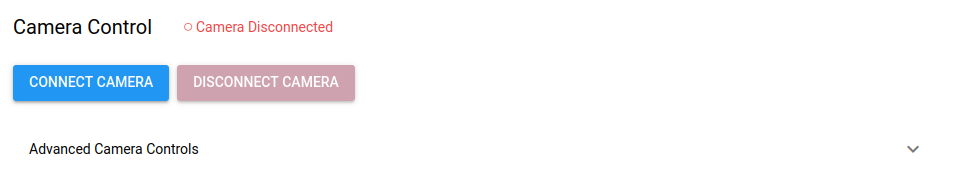
\includegraphics[width=1\textwidth]{Images/camera_control.png}
\caption{Camera control panel.}
\label{fig:ui_camera_control}
\end{figure}

\subsubsection{Datasets Panel}
The dataset panel enables handling captured images and related metadata. Users can import, create, select, and manage datasets, enabling systematic storage and categorization of images. Each image is linked to a specific scenario, allowing users to structure their tests based on various lens properties. Metadata embedding ensures that all relevant information, including camera settings and capture details, is preserved for future reference. The system also supports structured file naming conventions and temporary storage management, ensuring consistency and ease of navigation.

\begin{figure}[h]
\centering
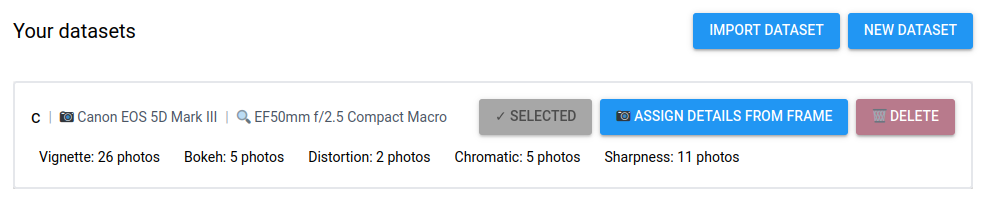
\includegraphics[width=1\textwidth]{Images/datasets_panel.png}
\caption{Datasets panel.}
\label{fig:ui_datasets}
\end{figure}

\subsubsection{Scenarios Panel} % todo
The scenarios panel allows users to target lens evaluations to specific properties, such as sharpness, vignetting, distortion, chromatic aberrations, and bokeh. Each scenario is linked to a dataset and includes predefined settings and workflows for capturing and analyzing images.

\begin{figure}[hbt]
\centering
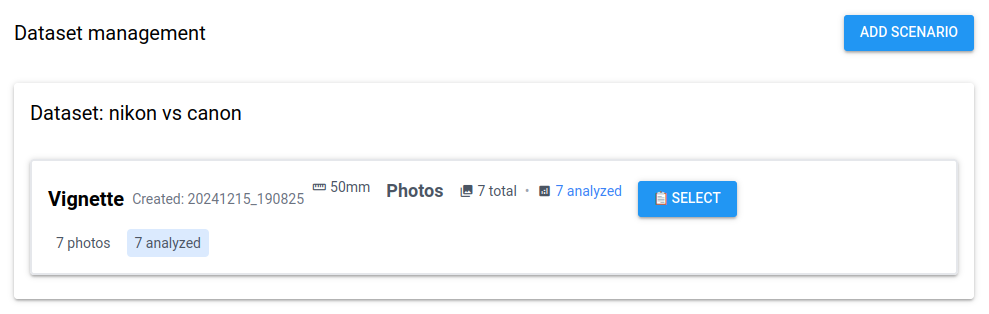
\includegraphics[width=1\textwidth]{Images/scenarios_panel.png}
\caption{Scenarios panel.}
\label{fig:ui_scenarios}
\end{figure}

The user can view detailed analysis results presented in a structured format. At the top, the Capture Settings section summarizes the camera configuration during the image capture. This includes details such as the camera model, lens information, aperture setting, shutter speed, ISO sensitivity, and focal length. These settings provide context for understanding the conditions under which the analysis was performed.

\begin{figure}[hbt]
\centering
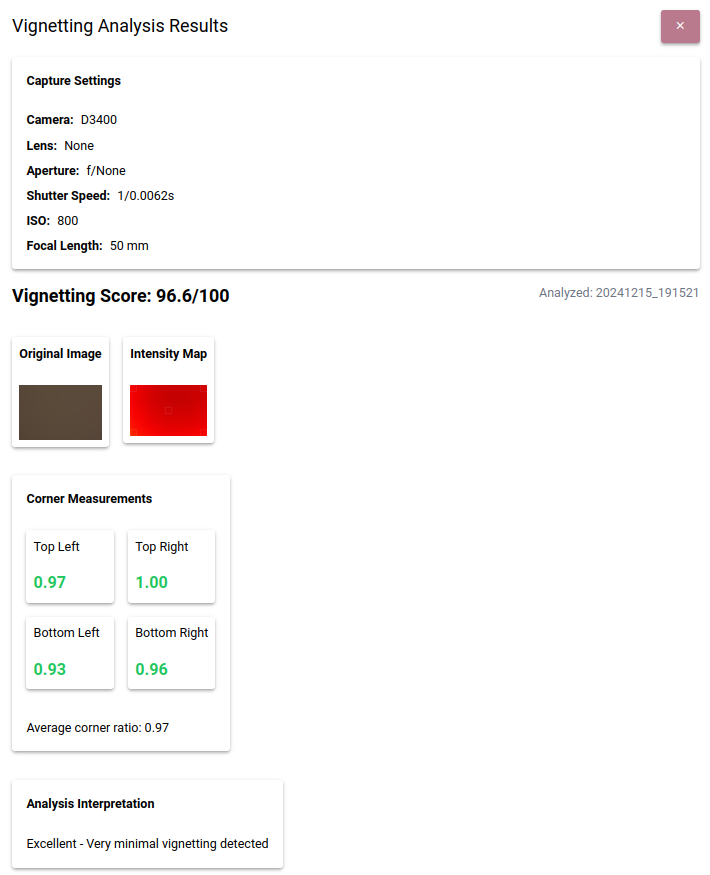
\includegraphics[height=0.8\textwidth]{Images/scenario_result.png}
\caption{Result of vignette scenario.}
\label{fig:ui_scenario_result}
\end{figure}

The Numerical Scores section delivers a quantitative assessment tailored to the specific scenario. For example, in sharpness analysis, this may include metrics like Modulation Transfer Function (MTF) scores. These scores are often normalized to a scale (e.g., 0-100) to simplify interpretation and enable comparisons across different lenses and settings.

The Visual Outputs section includes graphical representations to enhance the understanding of the analysis results. This may involve the display of the original captured image alongside processed visualizations, such as heatmaps, intensity maps and edge overlays.

The Measurement Details section provides more granular insights. This could include corner measurements for luminance ratios in vignetting analysis or edge intensity values for sharpness.

Finally, the Analysis Interpretation section summarizes the findings in plain language, offering a qualitative assessment of the results. For example, it may indicate whether vignetting is minimal, sharpness is excellent, or distortions are significant. This summary helps users quickly grasp the outcome of the analysis without needing to interpret the raw data or metrics.



\textbf{Vignetting} analysis results include center-to-corner luminance ratios, average corner intensity and a normalized vignetting score. Heatmaps visually represent brightness variations across the image and offer further insights into the vignetting effect.

\begin{figure}[hbt]
\centering

\includegraphics[width=0.4\textwidth]{Images/vignette_image_result.png}
\caption{Intensity map for vignette scenario.}
\label{fig:ui_vignette_intensity_map}
\end{figure}

For \textbf{sharpness} analysis, the UI displays numerical metrics such as Modulation Transfer Function (MTF) scores, edge intensity, and an overall sharpness rating. These are accompanied by graphs illustrating MTF curves across spatial frequencies and edge detection overlays that highlight areas of detail within the image. Original and processed images are shown side by side, providing clear visual comparisons.

\begin{figure}[h]
\centering
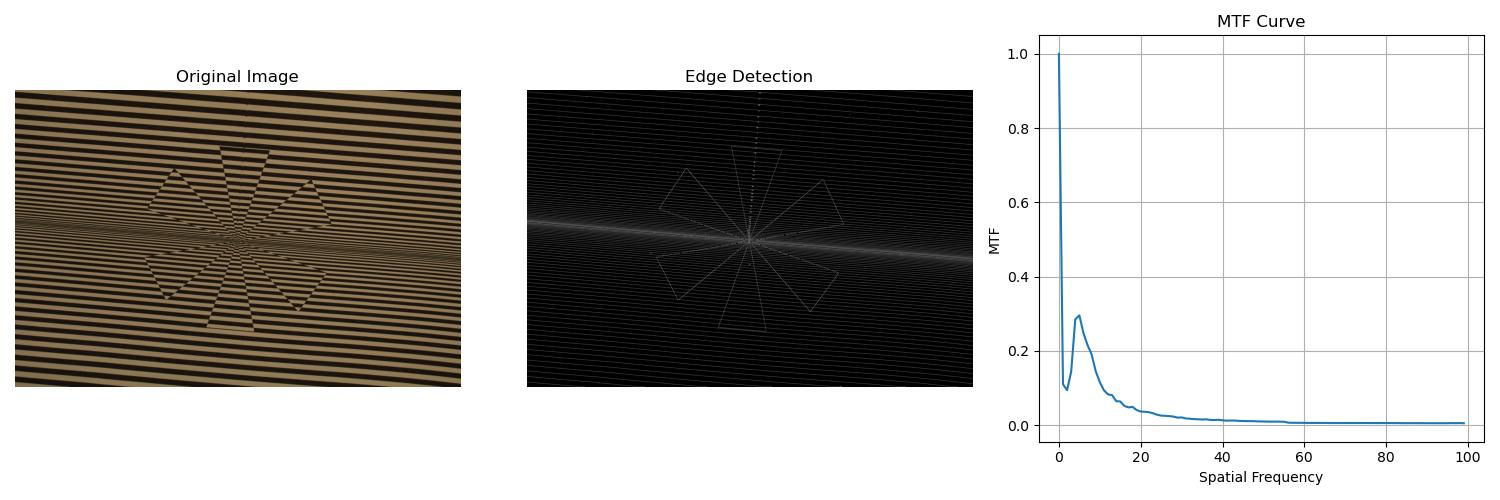
\includegraphics[width=1\textwidth]{Images/sharpness_image_result.jpg}
\caption{Sharpness analysis details.}
\label{fig:ui_sharpness_image}
\end{figure}

For \textbf{distortion} analysis, the system outputs metrics such as deviations in line straightness, average line deviation, and an overall distortion score. Grid overlays on the original image demonstrate detected distortion patterns, while corrected and uncorrected versions are displayed for comparison. The type of distortion—barrel, pincushion, or waveform—is identified based on the analysis.

\textbf{Chromatic aberration} analysis highlights color fringing in images, providing metrics on pixel offsets and scores for lateral and longitudinal aberrations. The UI displays zoomed-in sections of the image where chromatic aberrations occur, with overlaid color error vectors for visualization. Original and corrected images are presented side by side to showcase the impact of corrections.

In \textbf{bokeh} analysis, the system evaluates characteristics such as roundness, smoothness, and consistency of out-of-focus highlights. Overlays highlight bokeh regions, accompanied by metrics for size, shape, and edge definition. Users can compare bokeh characteristics across different aperture settings or light sources using dynamic visualization tools.

\begin{figure}[h]
\centering
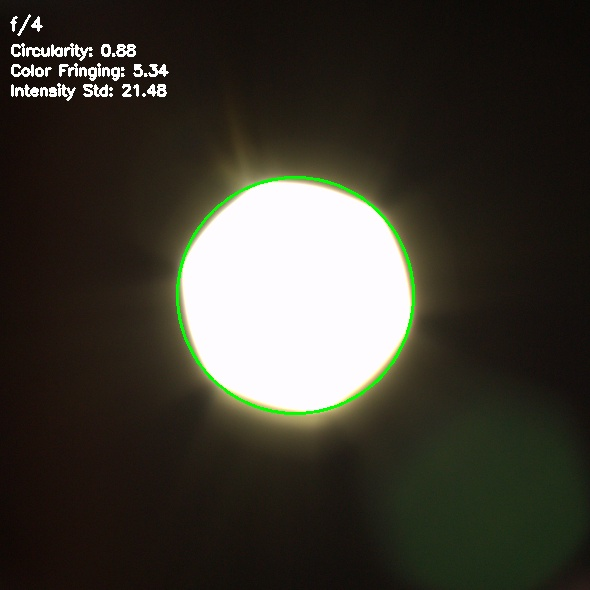
\includegraphics[width=0.3\textwidth]{Images/bokeh_image_result.jpg}
\caption{Bokeh analysis details.}
\label{fig:ui_bokeh_image}
\end{figure}

\subsubsection{System Logs}
The system logs provide a real-time record of application activities, ensuring transparency and aiding in troubleshooting. Logs capture key events such as camera connections, configuration changes, capture processes, and errors. Displayed within the user interface, the logs update dynamically, allowing users to monitor the status of ongoing tasks.

\begin{figure}[h]
\centering
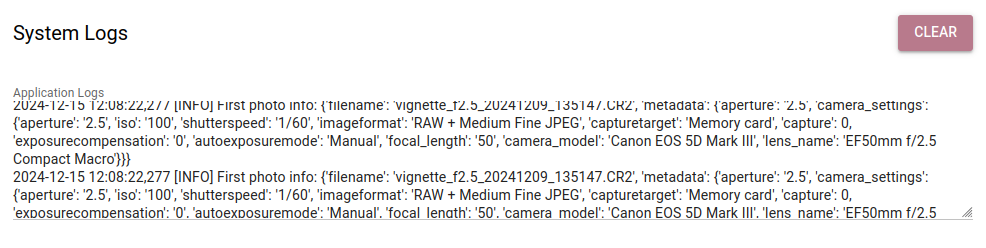
\includegraphics[width=1\textwidth]{Images/system_logs.png}
\caption{System logs.}
\label{fig:ui_system_logs}
\end{figure}

\subsubsection{Notifications}
The notification system provides real-time feedback to users. Notifications appear dynamically within the user interface to report critical events, such as successful camera connections and image captures. They also alert users to errors, including connection failures, invalid configurations, or file transfer issues.

\begin{figure}[h]
\centering

\includegraphics[width=0.7\textwidth]{Images/notification.png}
\caption{Notification example.}
\label{fig:ui_notification}
\end{figure}

%% BIG IMAGES
\begin{figure}[hbt]
\centering
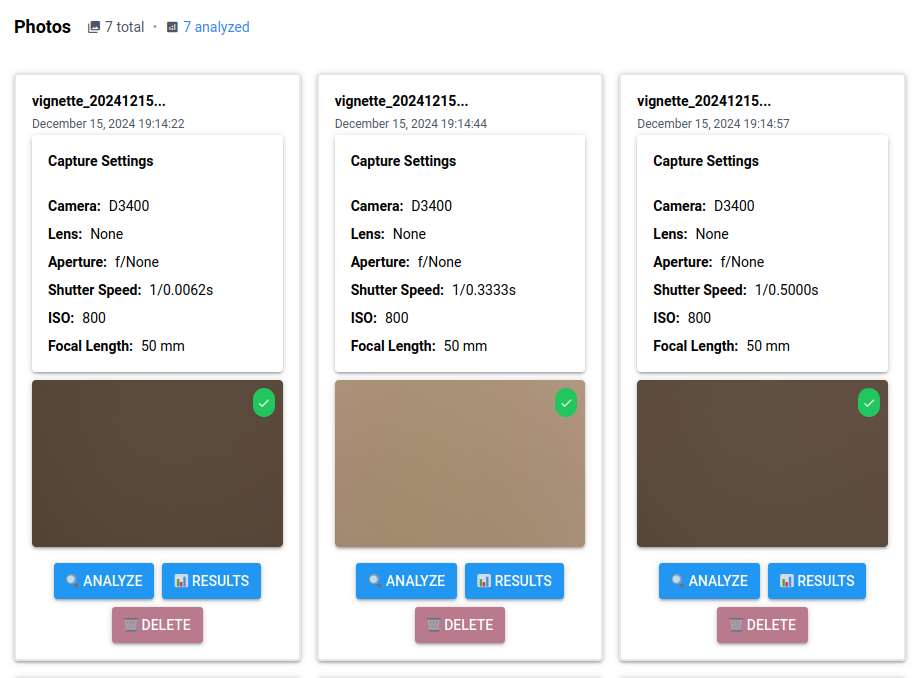
\includegraphics[width=0.8\textwidth]{Images/scenario_photos.png}
\caption{Overview of scenario's images.}
\label{fig:ui_scenario_images}
\end{figure}

\section{Testing}

To ensure the reliability and correctness of the application, particularly in the context of the "garage lab" approach described in the methodology, a comprehensive test suite was implemented using the pytest framework. The tests were designed to validate both the technical functionality and the practical usability of the application.

\subsection{Test Architecture}
The test suite is organized into four main components, reflecting the modular architecture of the application:
\begin{itemize}
    \item \texttt{test\_camera\_manager.py} - Validates camera control and image acquisition
    \item \texttt{test\_dataset\_manager.py} - Ensures proper data organization and persistence
    \item \texttt{test\_analysis.py} - Verifies image processing and lens measurement algorithms
    \item \texttt{test\_ui.py} - Tests user interface components and interactions
\end{itemize}

\subsection{Camera Manager Tests}
The camera manager tests focus on ensuring reliable camera operation in various scenarios:
\begin{itemize}
    \item Camera initialization and connection management
    \item Image capture and metadata extraction
    \item Camera configuration for different testing scenarios
    \item EXIF data processing for lens information
    \item Error handling and recovery mechanisms
\end{itemize}

Example of camera initialization test:
\begin{lstlisting}[language=Python]
def test_initialize_camera(mock_camera):
    """Test camera initialization"""
    with patch('gphoto2.Camera') as mock_camera_class:
        mock_camera_class.return_value = mock_camera
        mock_camera_class.autodetect = MagicMock(
            return_value=[(0, "Test Camera")])
        
        # Mock camera status check
        config = MagicMock()
        widget = MagicMock()
        widget.get_value.return_value = 0
        config.get_child_by_name.return_value = widget
        mock_camera.get_config.return_value = config
        
        manager = CameraManager()
        success = manager.initialize_camera()
        
        assert success
        assert manager.connected
        assert manager.camera is not None
\end{lstlisting}

\subsection{Analysis Tests}
The analysis tests verify the accuracy of lens measurement algorithms:
\begin{itemize}
    \item MTF calculation and sharpness analysis
    \item Bokeh quality assessment
    \item Distortion measurement
    \item Vignetting analysis
    \item Chromatic aberration detection
\end{itemize}

\subsection{UI Tests}
The UI tests ensure proper user interaction and workflow:
\begin{itemize}
    \item Camera connection and status display
    \item Test scenario execution
    \item Dataset and measurement management
    \item Result visualization and export
\end{itemize}

Example of photo capture test:
\begin{lstlisting}[language=Python]
def test_handle_capture_photo(ui_instance, temp_dir):
    """Test photo capture handling"""
    capture_result = {
        'path': os.path.join(temp_dir, "test.jpg"),
        'metadata': {
            'camera_settings': {
                'aperture': '1.8',
                'shutterspeed': '1/100',
                'iso': '400'
            }
        }
    }
    
    ui_instance.camera_manager.capture_image = MagicMock(
        return_value=capture_result)
    ui_instance.camera_manager.connected = True
    
    with patch('nicegui.ui.notify') as mock_notify:
        ui_instance.handle_capture_photo()
        ui_instance.camera_manager.capture_image\
            .assert_called_once()
        mock_notify.assert_called_once()
\end{lstlisting}

\subsection{Test Fixtures and Mocking}
To support the "garage lab" testing approach while ensuring reliable software testing:

\textbf{Test Fixtures}
\begin{itemize}
    \item \texttt{mock\_camera} - Simulates camera behavior
    \item \texttt{mock\_camera\_manager} - Provides camera control testing
    \item \texttt{temp\_dir} - Manages test file storage
    \item \texttt{dataset\_manager} - Handles test data organization
    \item \texttt{sample\_image} - Provides standardized test images
\end{itemize}

\textbf{External Dependencies}
\begin{itemize}
    \item Camera operations are mocked to ensure consistent testing
    \item File system operations are isolated for reproducibility
    \item UI components are simulated for interaction testing
    \item Image processing operations use controlled test data
\end{itemize}

\subsection{Quality Assurance}
The test suite ensures quality across several dimensions:

\textbf{Functional Testing}
\begin{itemize}
    \item Camera control reliability
    \item Data management accuracy
    \item Analysis algorithm precision
    \item UI responsiveness and usability
\end{itemize}

\textbf{Error Handling}
\begin{itemize}
    \item Camera connection issues
    \item Invalid user input
    \item Resource availability
    \item Data corruption scenarios
\end{itemize}

\textbf{Performance Testing}
\begin{itemize}
    \item Image processing efficiency
    \item Memory usage optimization
    \item Response time measurement
    \item Resource cleanup verification
\end{itemize}

Test coverage reports are generated using pytest-cov to ensure comprehensive testing of all components, with particular attention to critical paths in the lens measurement workflows.

\subsection{Application Features}
The application includes several key features that enhance user experience and functionality:
\begin{itemize}
    \item \textbf{Offline Operation}: The application can operate fully offline after the initial installation, allowing users to utilize its features without internet connectivity.
    \item \textbf{Dark Mode}: The application includes a dark mode feature, enhancing usability in low-light environments and providing a more comfortable viewing experience.
    \item \textbf{UI State Storage}: The application stores user interface state, including user preferences and the currently opened elements, between visits, ensuring a seamless user experience.
\end{itemize}
